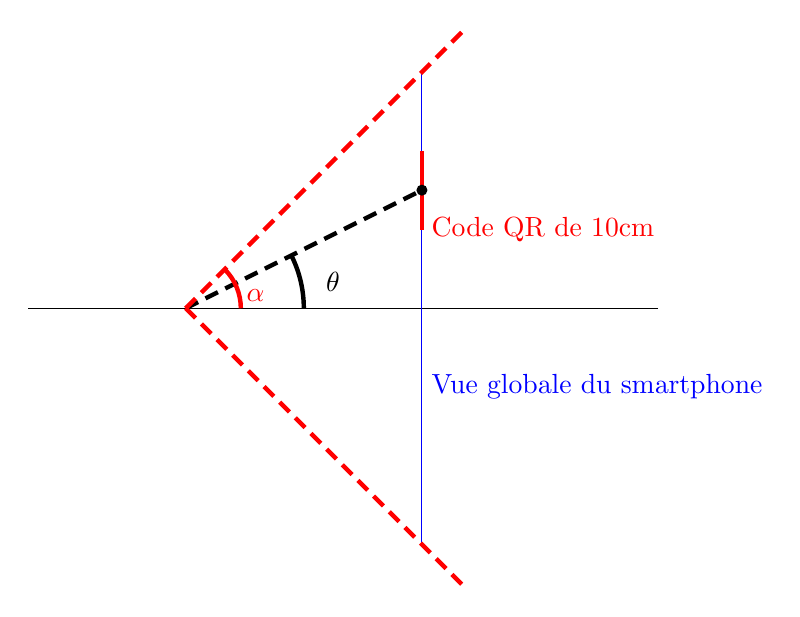
\begin{tikzpicture}

    % define coordinates
    \coordinate (O) at (0,0) ;
    \coordinate (A) at (6,0) ;
    \coordinate (B) at (-2,0) ;

    \coordinate (E) at (3,3) ;
    \coordinate (F) at (3,-3) ;
    
   \coordinate (A_QR_R) at (3,1) ;
   \coordinate (B_QR_R) at (3,2) ;
   \coordinate (M_QR_R) at (3,1.5) ;
   
   



    % axis
    \draw[] (A) -- (B) ;
    

      \draw[blue] (E) -- (F) ;
      \draw[red,ultra thick] (A_QR_R) -- (B_QR_R) ;
      \node[right,red] at (3,1){Code QR de 10cm};
        \node[right,blue] at (3,-1){Vue globale du smartphone};
      
      \fill[black] (M_QR_R) circle (2pt);
      \draw[dash pattern=on5pt off3pt,ultra thick] (O) -- (M_QR_R) ;



    % rays
    \draw[dash pattern=on5pt off3pt,red,ultra thick] (O) -- (45:5);
    \draw[dash pattern=on5pt off3pt,red,ultra thick] (O) -- (-45:5);

    % angles
    \draw[ultra thick,red] (0.7,0) arc (0:45:0.7);
        \draw[ultra thick,black] (1.5,0) arc (0:26:1.5);
    \node[black] at (10:1.9)  {$\theta$};

    \node[red] at (10:0.9)  {$\alpha$};
    
    
\end{tikzpicture}